\documentclass[11pt,a4paper]{beamer}
\usepackage[latin1]{inputenc}
\usepackage[dutch]{babel}

\usepackage[absolute,overlay]{textpos}
\setlength{\TPHorizModule}{1mm}
\setlength{\TPVertModule}{1mm}

\author{Zeus WPI}

% Voor- en achtergrondkleurtjes
\definecolor{gray}{RGB}{56,56,56}
\setbeamercolor{background canvas}{bg=gray}
\setbeamercolor{normal text}{fg=white}
\setbeamercolor{block title}{fg=white}
% Verwijder navigatieknopjes
\beamertemplatenavigationsymbolsempty

% Randjes voor fbox's rond de afbeeldingen
\setlength{\fboxsep}{0pt}
\setlength{\fboxrule}{1pt}


\begin{document}

% Eerste slide met logo
\begin{frame}
  
\includegraphics[width=\textwidth]{zeus_logo.pdf}\\[5mm]

  \hfill --- by Procrat \&\& Basho

  \note{Wij komen Zeus WPI voorstellen. Zeus is een werkgroep van studenten,
    voornamelijk voor mensen uit onze richting en iedereen ge\"interesseerd is
    in informatica.}
\end{frame}


% Wat we doen
\begin{frame}
  \begin{textblock}{20}(10,25)
    {\Huge Activiteiten}
  \end{textblock}

  \pause
  \begin{textblock}{20}(50,45)
    \visible<2->{\Huge Projecten}
  \end{textblock}

  \pause
  \begin{textblock}{20}(90,65)
    \visible<3->{\Huge Sfeer}
  \end{textblock}

  \note{We voorzien met Zeus in principe drie zaken: enerzijds zorgen we voor
    wekelijkse activiteiten, ten tweede werken we mee aan verschillende
    projecten en ten slotte zorgen we ook gewoon voor een gezellige sfeer.}
\end{frame}


% Activiteiten
\begin{frame}
  \begin{center}
    {\Huge Activiteiten}
  \end{center}

  \note{Vanaf dit jaar zullen we iedere week een activiteit houden. Dit kan
    van verscheidene aard zijn.}

  \pause
  \begin{textblock}{20}(3,45)
    \visible<2->{\fbox{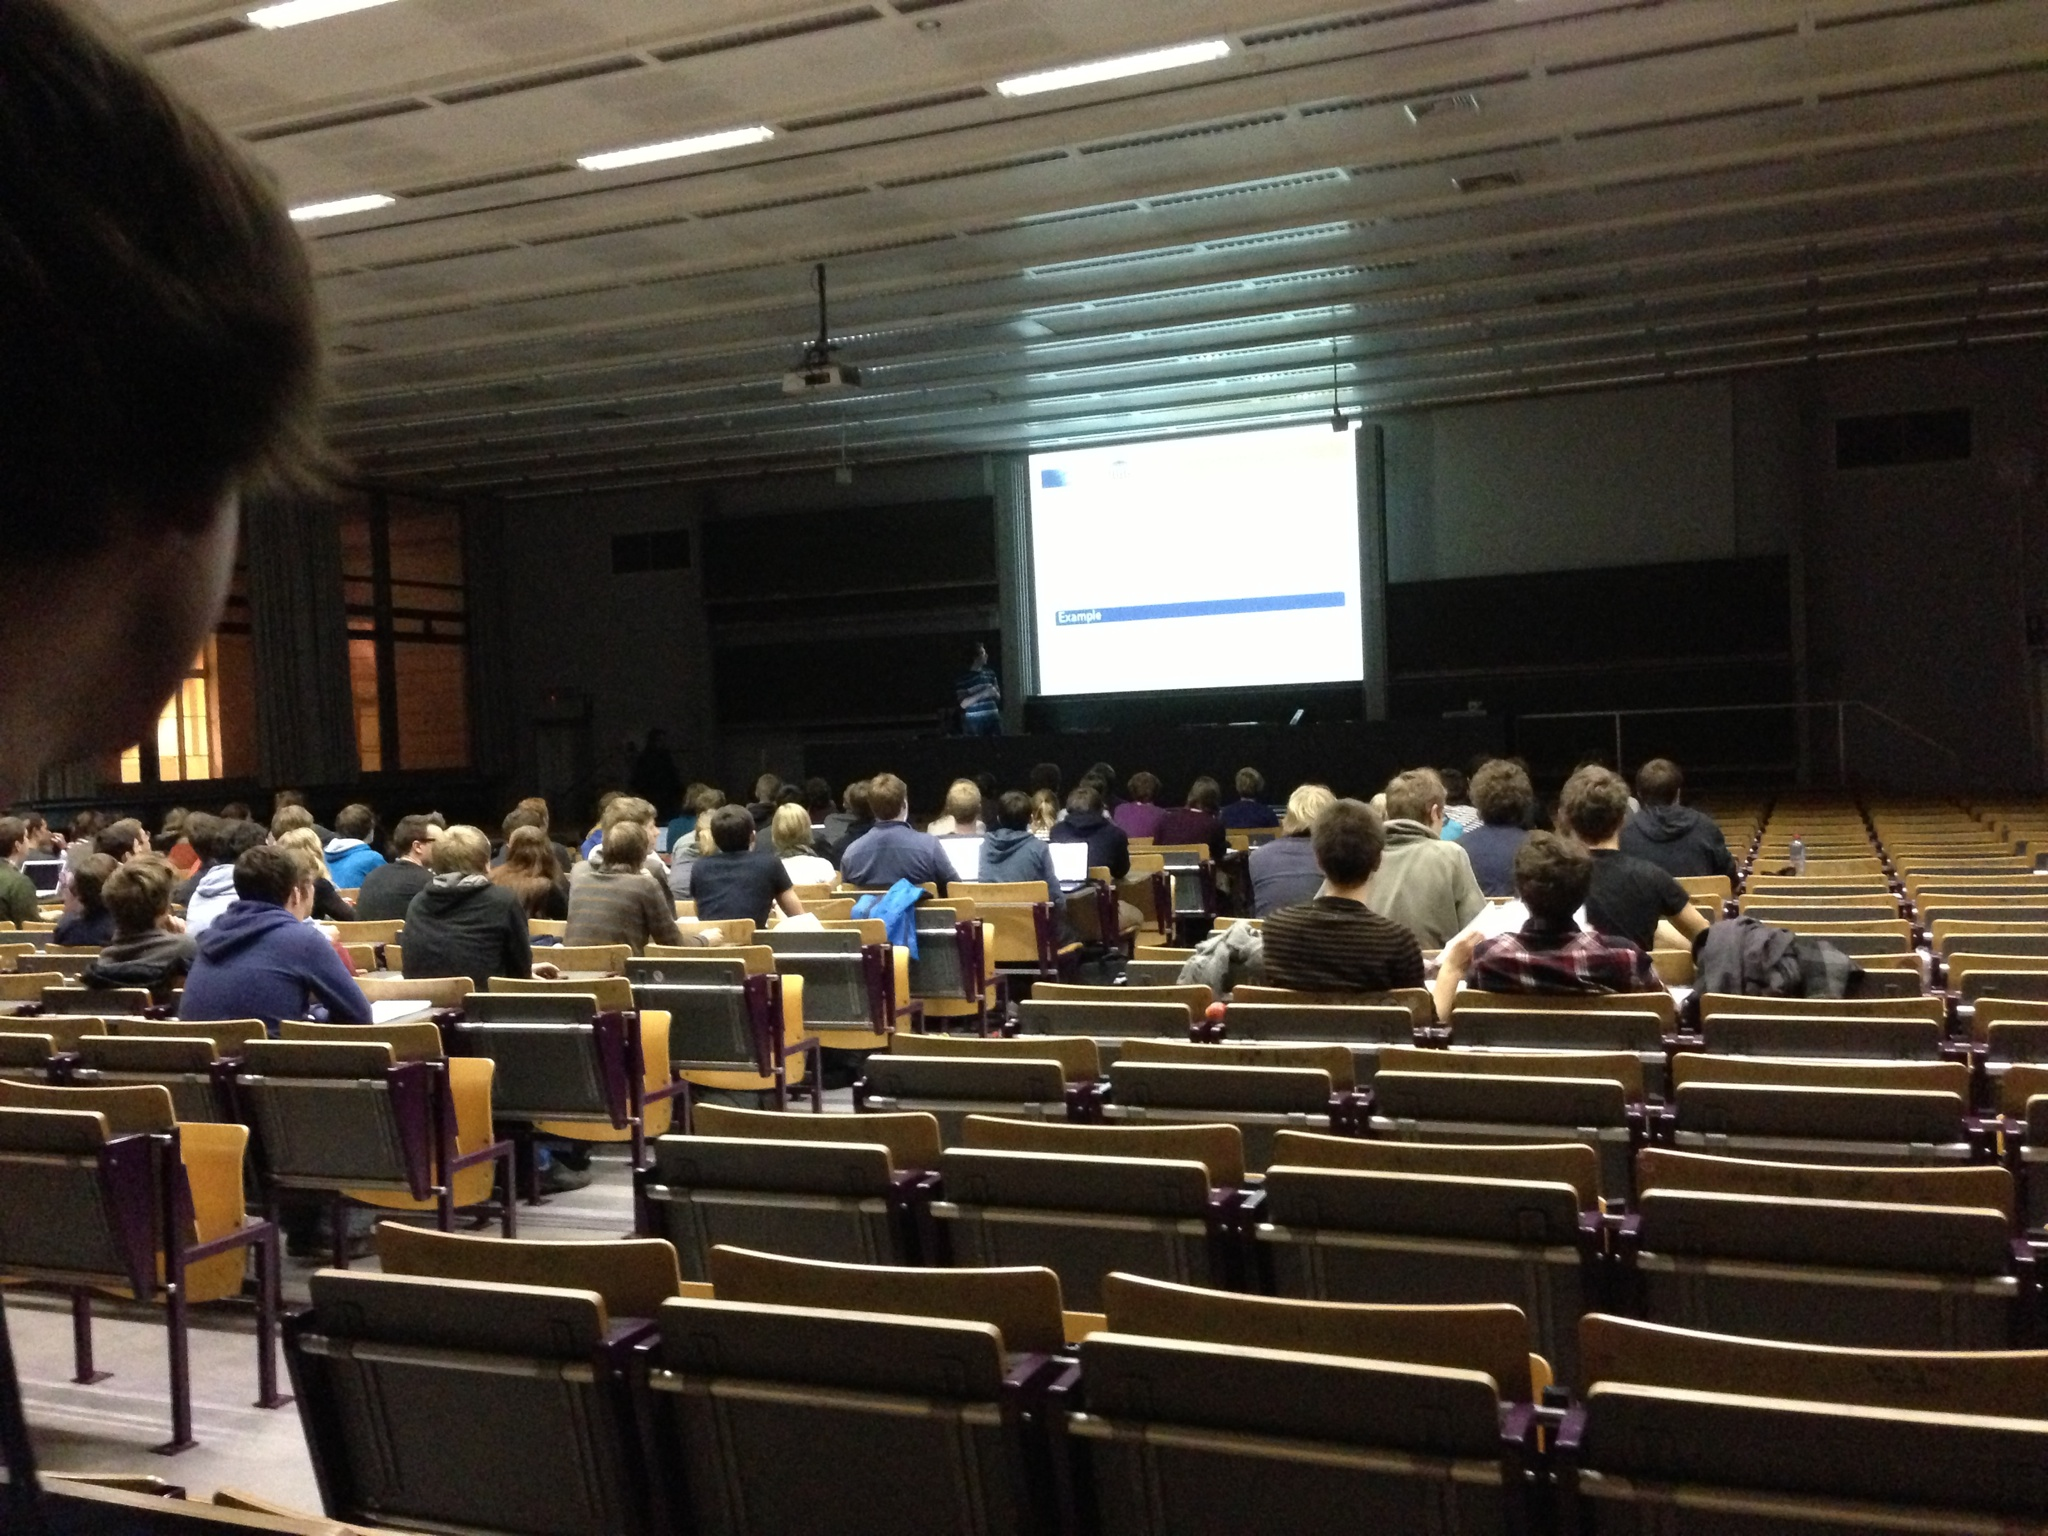
\includegraphics[width=180pt]{activiteit_latex.jpg}}}
  \end{textblock}

  \note<2->{Zo geven heel wat talks en introductielessen. Dit semester zijn dat
    een \LaTeX-les, een JS/D3-les, een Haskell-teaser, een Ruby-les en een
    Rails-les. Maak je geen zorgen als sommige namen je nog niets zeggen. In
    het tweede semester geven we ook een Git-les en een Python-les, maar zullen
    we ook verder gaan dan introductielessen en de opgedane kennis toepassen in
    geavanceerdere lessen.}

  \pause
  \begin{textblock}{20}(22,30)
    \visible<3->{\fbox{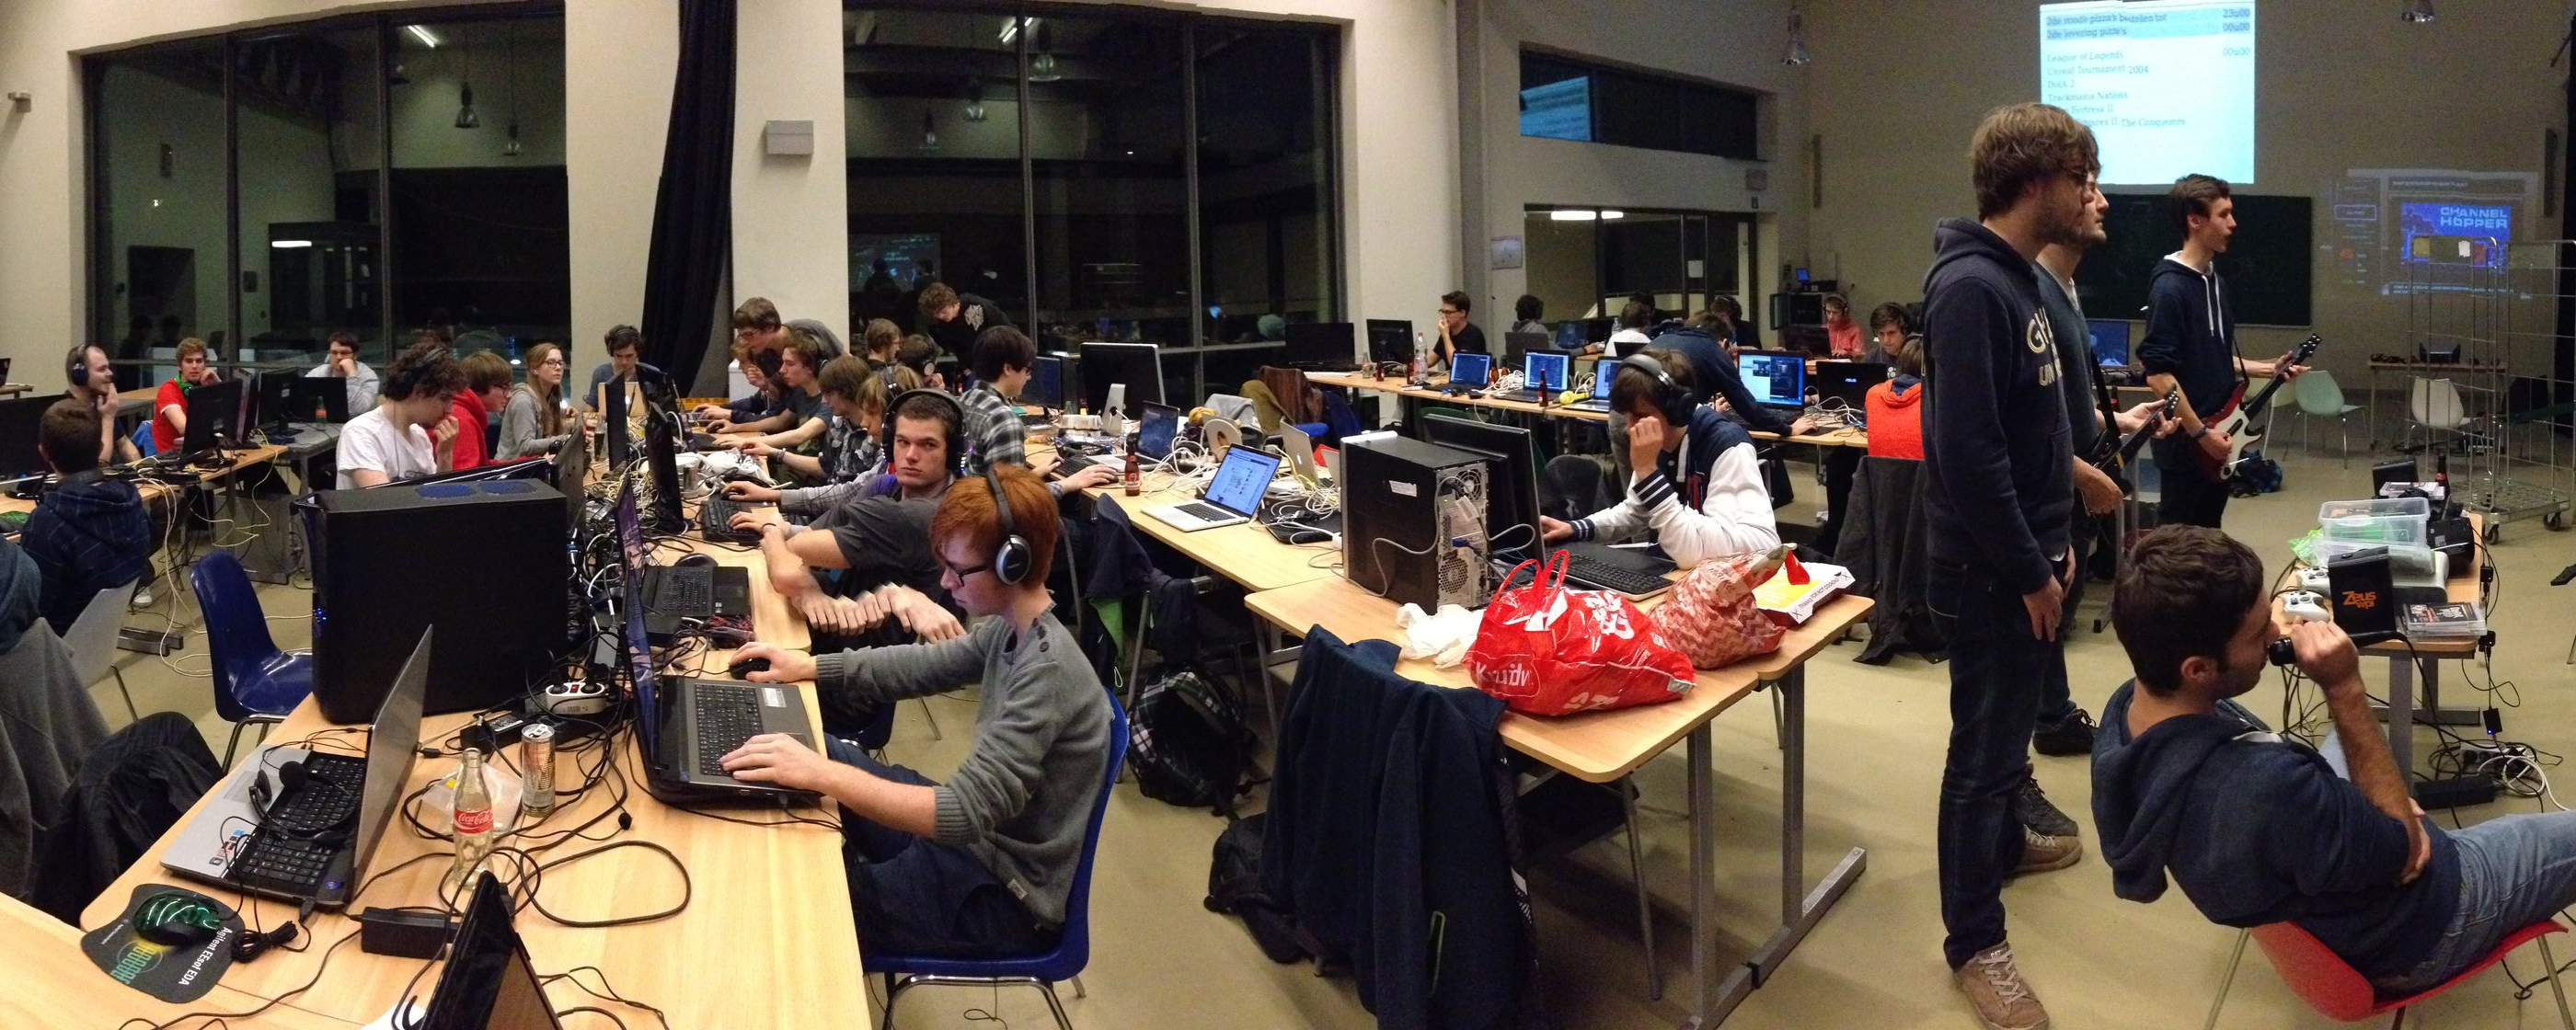
\includegraphics[width=235pt]{activiteit_lan.jpg}}}
  \end{textblock}

  \note<3->{Onze activiteiten zijn niet allemaal even serieus. We houden
    jaarlijks een 24h-LAN-party waar steeds meer en meer mensen op afkomen. We
    zullen dit semester ook enkele spelletjesavonden organiseren.}

  \pause
  \begin{textblock}{20}(41,3)
    \visible<4->{\fbox{\includegraphics[width=230pt]{activiteit_codenight.jpeg}}}
  \end{textblock}

  \note<4->{Ongeveer iedere week zullen we codenights houden. Je bent welkom om
    mee te helpen aan een van onze vele projecten, om op je eentje wat te
    programmeren of gewoon mee de sfeer cre\"eren.}

  % 2e semester
  \pause
  \begin{textblock}{20}(10,10)
    \visible<5->{\fbox{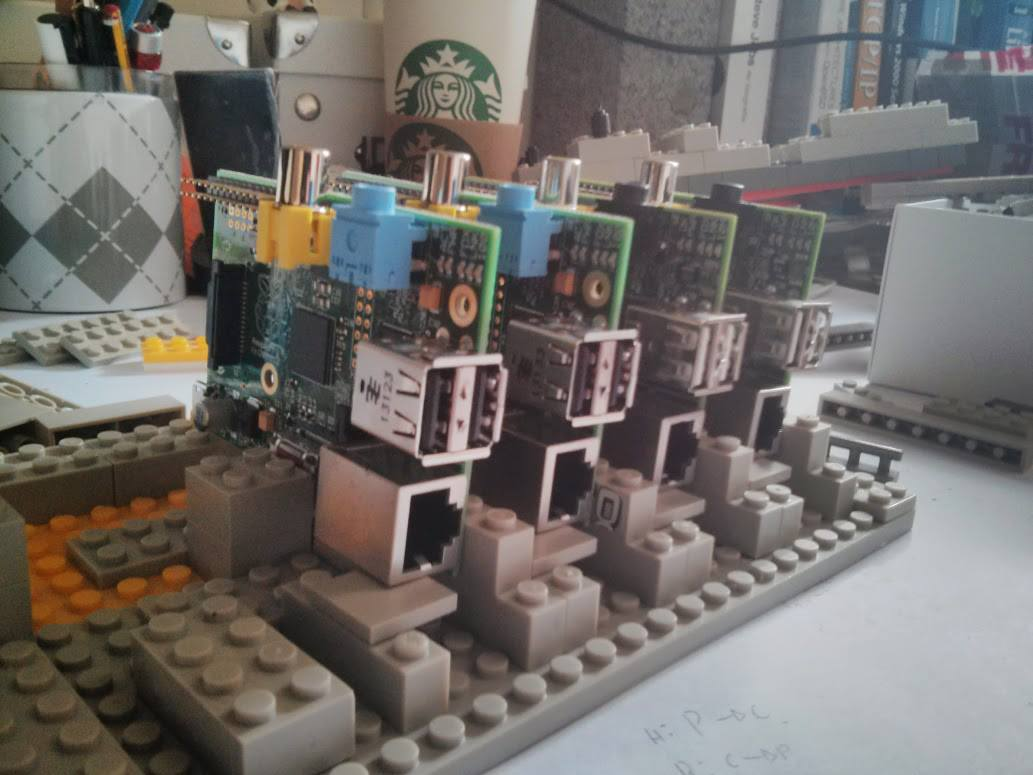
\includegraphics[width=180pt]{activiteit_hwavond.jpg}}}
  \end{textblock}

  \note<5->{In het tweede semester houden we misschien een hardware-avond
    houden. Dat is eigenlijk een avondje prutsen met lego, raspberry-pi's en
    een paar circuitjes.}

  \pause
  \begin{textblock}{20}(54,50)
    \visible<6->{\fbox{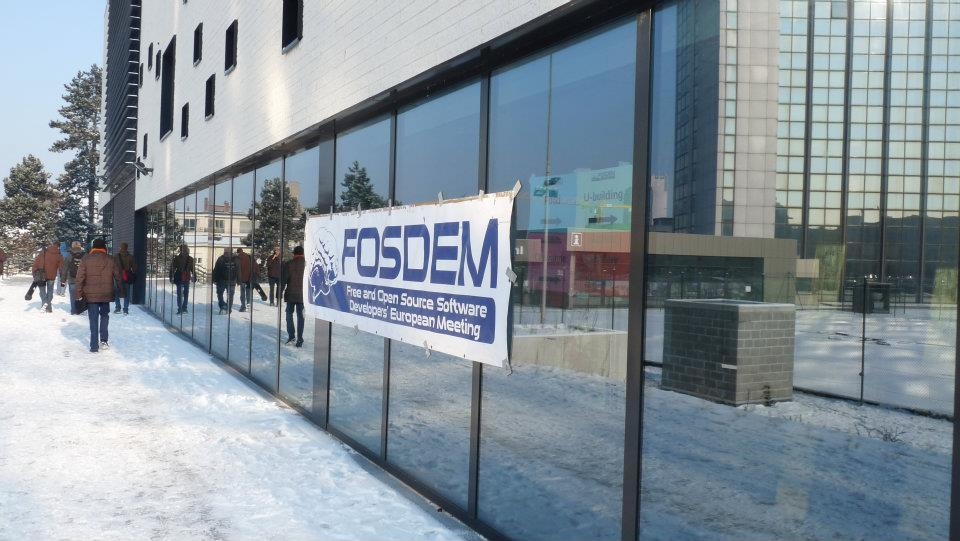
\includegraphics[width=180pt]{activiteit_fosdem.jpg}}}
  \end{textblock}

  \note<6->{Soms verlaten we ons eigen terrein echter en trekken we naar
    grotere evenementen, zoals FOSDEM, een open source meeting in Brussel en
    naar de Vlaamse Programmeerwedstrijd. Maar dit is ook voor het tweede
    semester.}

  \pause
  \begin{textblock}{20}(5,5)
    \visible<7->{\fbox{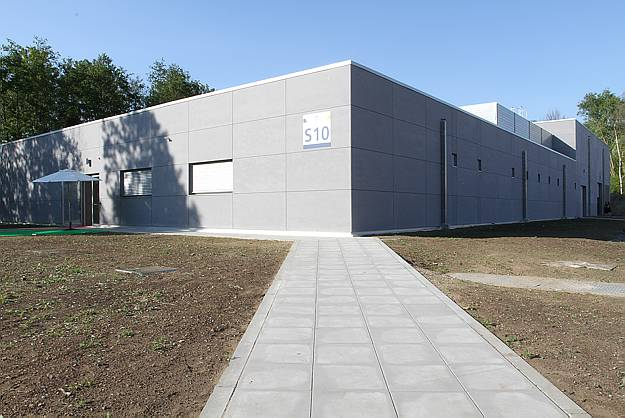
\includegraphics[width=180pt]{activiteit_datacenter1.jpg}}}
  \end{textblock}
  \begin{textblock}{20}(58,35)
    \visible<7->{\fbox{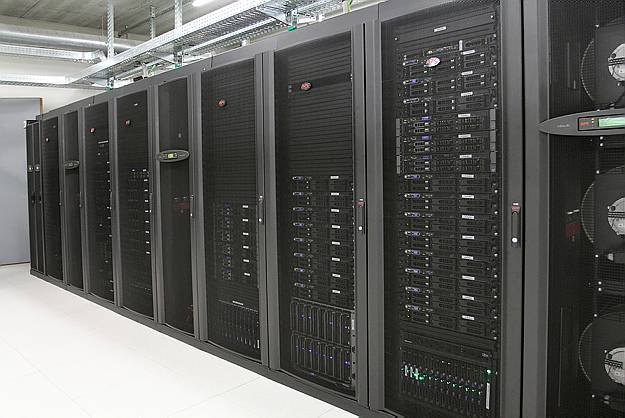
\includegraphics[width=180pt]{activiteit_datacenter2.jpg}}}
  \end{textblock}

  \note<7->{Volgende week donderdag starten we al met een bezoek aan S10. Daar
    bevindt zich het datacenter van UGent en de eerste tier-1 supercomputer van
    Vlaanderen.}
\end{frame}

% Projecten
\begin{frame}
  \begin{center}
    {\Huge Projecten}
  \end{center}

  \note{Zoals ik al zei houden we ons met heel wat projecten bezig.}

  \pause
  \begin{textblock}{20}(3,3)
    \visible<2->{\fbox{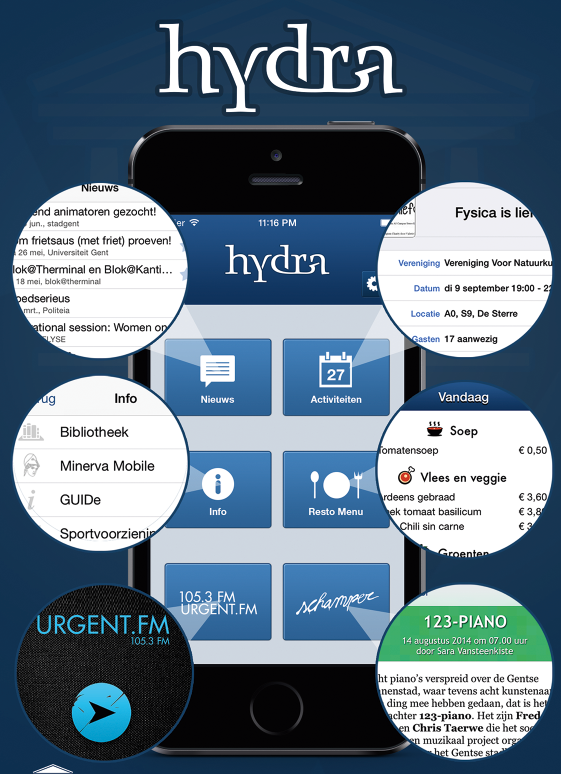
\includegraphics[width=180pt]{project_hydra.png}}}
  \end{textblock}

  \note<2->{We hebben onder andere een tijdje geleden Hydra geschreven, de
    studentenapp van UGent. We onderhouden deze nog steeds.}

  \pause
  \begin{textblock}{20}(15,25)
    \visible<3->{\fbox{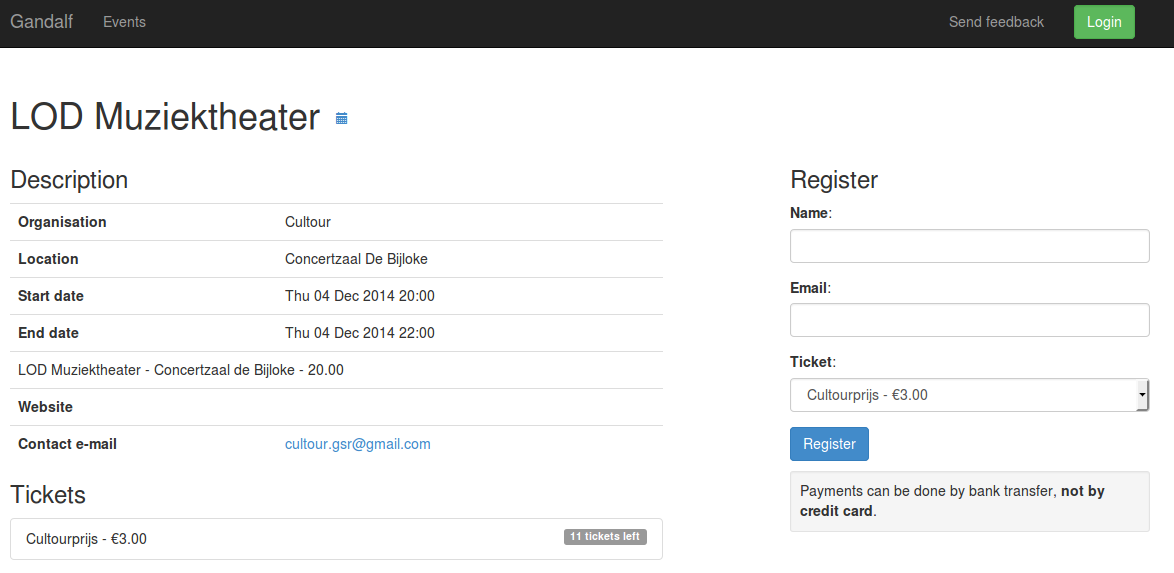
\includegraphics[width=270pt]{project_gandalf.png}}}
  \end{textblock}

  \note<3->{We hebben ook een event- en ticketingsysteem geschreven voor de
    overkoepelende vereniging van studentenverenigingen.}

  \pause
  \begin{textblock}{20}(41,8)
    \visible<4->{\fbox{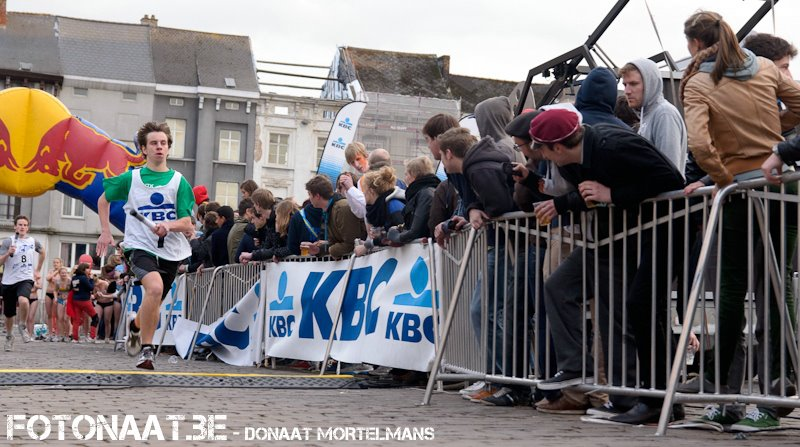
\includegraphics[width=230pt]{project_12ul.jpg}}}
  \end{textblock}

  \note<4->{Ieder jaar verzorgen we het automatisch telsysteem op de
    12-urenloop, met bijhorende website.}

  \pause
  \begin{textblock}{20}(8,45)
    \visible<5->{\fbox{\includegraphics[width=180pt]{project_slotmachien}}}
  \end{textblock}

  \note<5->{Dit jaar hebben we ook een systeem gemaakt om de deur van
    onze kelder van op afstand open te doen.}

  \pause
  \begin{textblock}{20}(37,35)
    \visible<6->{\fbox{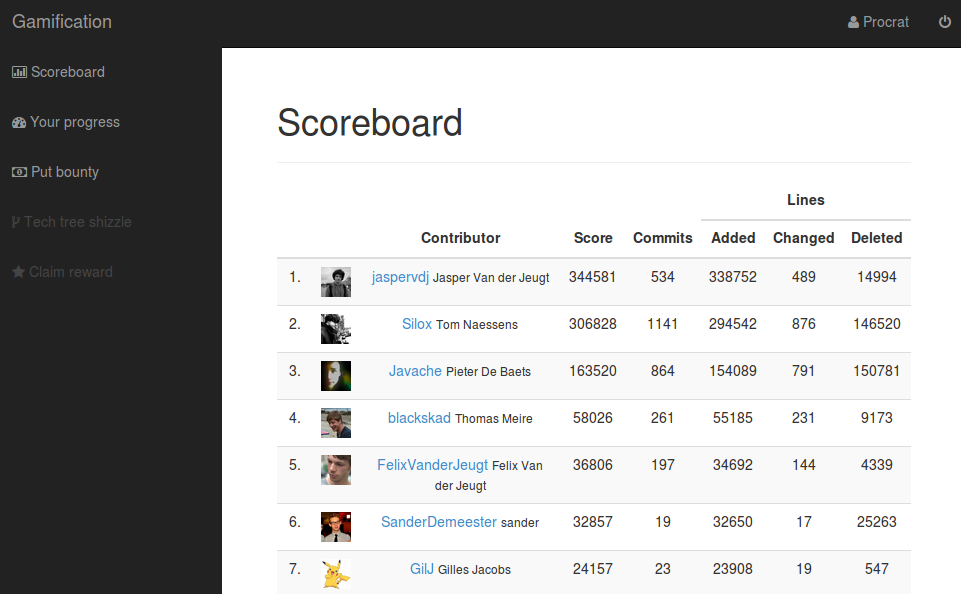
\includegraphics[width=230pt]{project_gamification.png}}}
  \end{textblock}

  \note<6->{We hebben daarnaast nog wat kleinere projectjes of projecten die
    niet in \'e\'en zin uit te leggen zijn. Zoals je ziet zijn we met heel wat
    verschillende dingen bezig!}
\end{frame}

% Kelder
\begin{frame}
  \begin{center}
    {\Huge{Zeus Kelder}}\\[5mm]

    \hspace*{-230pt}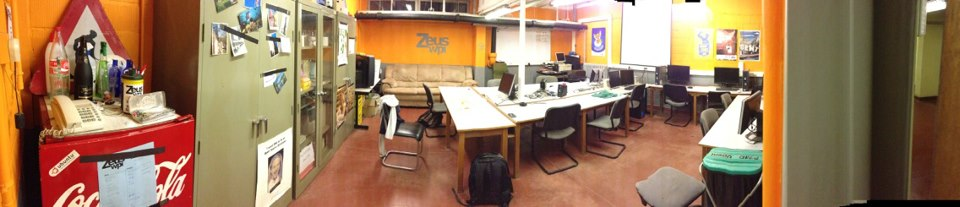
\includegraphics[width=700pt]{kelder.jpg}

    \bigskip 51.023102,3.710265 | Verdieping -1
  \end{center}

  \note{Voor wie zich nu zou afvragen waar dit zich allemaal afspeelt: wij
    hebben hier beneden een gezellige kelder, waar er tussen de lessen door
    en \'s avonds vaak volk zit. Straks kun je ons daar ook vinden dus kom
    gerust eens langs!}

  \note{Je zal nog van ons horen via posters of wanneer we langs komen in de
    lessen. Als je straks langskomt, kunnen we je ook inschrijven op onze
    mailinglijst zodat je altijd op de hoogte blijft van komende activiteiten.}
\end{frame}

\end{document}
